\documentclass[A4paper]{article}
\usepackage[a4paper, total={7.2in, 10.5in}]{geometry}
\usepackage{tikz}
\usetikzlibrary{calc}
\usepackage{setspace}
\usepackage{graphicx}
\usepackage{amsmath}
\usepackage{pgfplots}
\usepackage[hidelinks]{hyperref}
\usepackage{bookmark}
\DeclareMathOperator\cosec{cosec}

\graphicspath{ {./images/} }

\setlength{\parindent}{0pt}

\title{A Level Mathematics - Mechanics}
\author{Xingzhi Lu (2129570@concordcollege.org.uk)}
\date{2024}

\begin{document}
	\maketitle

	\section{Vectors}
	\subsection{Calculations}
	\begin{itemize}
		\item $\vec{a}=\vec{a_x}+\vec{a_y}$
		\item $|\vec{a_x}|=|\vec{a}|\cos\theta$
		\item $|\vec{a_y}|=|\vec{a}|\sin\theta$
		\item $\tan\theta = \dfrac{|\vec{a_y}|}{|\vec{a_x}|}$
		\item $|\vec{a}|^2=|\vec{a_x}|^2+|\vec{a_y}|^2$
		\item $\vec{a} \cdot \vec{b} = |\vec{a}||\vec{b}|\cos\theta = x_1x_2+y_1y_2$
		\begin{description}
			\item If $a\perp b$: $\vec{a} \cdot \vec{b} = 0$
		\end{description}
		\item $\cos \theta = \dfrac{\vec{a} \cdot \vec{b}}{|\vec{a}||\vec{b}|}$
		\item $\text{Unit vector (magnitude = 1)} = \dfrac{\vec{a}}{|\vec{a}|}$

	\end{itemize}
	\subsection{Find the resultant of two vectors}
	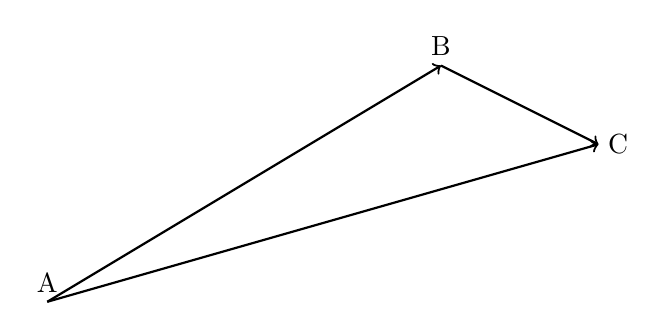
\begin{tikzpicture}
		\draw[->,thick] (0,0) -- (5,3);
		\draw[->,thick] (5,3) -- (7,2);
		\draw[->,thick] (0,0) -- (7,2);
		\node[above] at (0,0) {A};
		\node[above] at (5,3) {B};
		\node[right] at (7,2) {C};
	\end{tikzpicture}\\
	\\
	$\overrightarrow{AC}=\overrightarrow{AB}+\overrightarrow{BC}$\\
	$|\overrightarrow{AC}|$ can be found by sine or cosine rule

	\pagebreak

	\section{Forces and motion}
	\subsection{Types of motion}
	\subsubsection{Constant speed motion}
	\textbf{Calculations:}
	\begin{itemize}
		\item $v$ is constant, $a=0$
		\item $d=vt$
	\end{itemize}
	\textbf{Motion graphs:}
	\subsubsection{Uniform acceleration motion}
	\textbf{Calculations:}
	\begin{itemize}
		\item $d=v_it+\dfrac{1}{2}at^2$
		\item $v_f=v_i+at$
		\item $v_f^2=v_i^2=2as$
		\item $d=\overline{v}t$
		\item $\overline{v} = \dfrac{v_i+v_f}{2}$
	\end{itemize}
	\textbf{\textbf{Motion graphs:}}

	\subsubsection{Free fall}
	Air resistance is ignored, so $a=g$\\
	\textbf{Calculations:}
	\begin{itemize}
		\item $v_i = 0$
		\item $v_f = gt$
		\item $h=\dfrac{1}{2}gt^2$
	\end{itemize}
	\subsubsection{Vertically upward}
	\textbf{Calculations:}
	\begin{itemize}
		\item $v = u - gt$
	\end{itemize}
	Rising and falling at the same height: speed same, opposite direction
	\subsubsection{Projectile}
	\textbf{Calculations:}
	\begin{itemize}
		\item $y=\tan\theta x - \dfrac{g}{2u^2}(1+\tan^2\theta)x^2$
		\item range = $\dfrac{u^2\sin 2\theta}{g}$
		\item greatest height: $\dfrac{u^2\sin^2\theta}{2g}$
		\item Time to flight (back to x-axis) = $\dfrac{2u\sin\theta}{g}$
		\item Time to greatest height: $\dfrac{u\sin\theta}{g}$
	\end{itemize}
	\subsection{Types of forces}

	\pagebreak

	\section{Momentum}


	\pagebreak


	\section{Moments}
	\subsection{Definition}
	\textbf{Turning} effect of the force on a rigid body.\\
	Clockwise moment of $F$ about P: $|F|\times d= \vec{F}\times\vec{d} = |F||d|\sin\theta$
	\subsection{Right hand rule}
	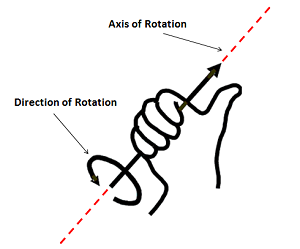
\includegraphics[width=0.4\textwidth]{rhr}\\
	$\vec{a} \times \vec{b}$= from $\vec{a}$ to $\vec{b}$\\
	$\vec{b} \times \vec{a}$= from $\vec{b}$ to $\vec{a}$
	

	\pagebreak

	\section{Common questions}
	\subsection{Projectile}
	\subsubsection{Asking for improvements}
	
	
	
	
	

\end{document}